\documentclass[12pt]{beamer}

\usetheme{Oxygen}
\usepackage[utf8]{inputenc}
\usepackage[english]{babel}
\usepackage{amssymb}
\usepackage{amsmath}
\usepackage{thumbpdf}
\usepackage{wasysym}
\usepackage{ucs}
\usepackage[utf8]{inputenc}
\usepackage{pgf,pgfarrows,pgfnodes,pgfautomata,pgfheaps,pgfshade}
\usepackage{verbatim}
\usepackage{xspace,framed,here,keystroke}
\usepackage{graphicx}
%\usepackage{minted} % Added highlighting in source code

% Enable/Disable notes - It creates a white complementary slide to help the presenter save the spech
%\setbeameroption{show notes}
%\setbeamertemplate{note page}[plain]

\setbeamertemplate {navigation symbols}{} % Remove buttons in footnote

\pdfinfo
{
  /Title       (Proposal: Translation of B Implementations to LLVM-IR)
  /Creator     (David Déharbe and Valério Medeiros)
  /Author      (David Déharbe and Valério Medeiros)
}


\title{Proposal: Translation of B Implementations to LLVM-IR}
%\subtitle{B2LLVM: A First Proposal }
\author{ D. B. P. Déharbe and V. G. Medeiros Jr. }
\date{October 2, 2013}


% Commands 

\newcommand{\trad}[2]{\ensuremath{\lVert \textsf{#1} \rVert^{\textit{#2}}}}
\newcommand{\nl}[0]{\text{\Return}}
\newcommand{\mty}[0]{\texttt{""}}
\DeclareMathOperator{\conc}{\diamond}
\DeclareMathOperator{\isdef}{\equiv}
\DeclareMathOperator{\dom}{\mbox{dom}}
\DeclareMathOperator{\name}{\mathcal{L}()}
\newcommand{\llvm}[1]{\texttt{#1}}
\newcommand{\B}[1]{\textsf{#1}}
\newcommand{\lalt}[0]{$\langle$\xspace}
\newcommand{\ralt}[0]{$\rangle$\xspace}
%\newcommand{\alt}[0]{$\mid\,$}
\newcommand{\ListOf}[1]{$\mbox{#1}^+$}
\newcommand{\nt}[1]{{\normalfont\textit{#1}}}
\newcommand{\Dict}[0]{\mathbb{D}}
\newcommand{\Text}[0]{\mathbb{T}}
\newcommand{\IF}[0]{\textbf{ if }}
\newcommand{\ELSIF}[0]{\textbf{ else if }}
\newcommand{\ELSE}[0]{\textbf{ else }}
\newcommand{\THEN}[0]{\textbf{ then }}
\newcommand{\LET}[0]{\textbf{ let }}
\newcommand{\IN}[0]{\textbf{ in }}
\newcommand{\AND}[0]{\textbf{ and }}
\newcommand{\PH}[1]{\framebox{$#1$}}
\newcommand{\sep}[0]{\otimes}
\newcommand{\intf}[0]{\ensuremath{\mathbb{I}}}
\newcommand{\Global}[0]{\ensuremath{\sf\Gamma}}
\newcommand{\local}[0]{\ensuremath{\sf\lambda}}
\newcommand{\opmap}[0]{\ensuremath{\sf\Omega}}
\newcommand{\idx}[0]{\ensuremath{\sf\Pi}}
\newcommand{\state}[0]{\ensuremath{\sf\Sigma}}
\newcommand{\tradi}[2]{\ensuremath{\langle \textsf{#1} \rangle^{\textit{#2}}}}




\begin{document}

% To enable numbered captions
\setbeamertemplate{caption}[numbered]

\frame{\titlepage}

%Show the first out line
%\section*{}
%\begin{frame}
%  \frametitle{Outline}
%  \tableofcontents[section=1,hidesubsections]
%  \note[item]{After that, I will; Following that, I will; Then, I will}
%\end{frame}

%Show the transition outline in each section
%\AtBeginSection[]
%{
%  \frame<handout:0>
%  {
%    \frametitle{Outline}
%    \tableofcontents[currentsection,hideallsubsections]
%  }
%}

%Show the transition outline in each subsection
%\AtBeginSubsection[]
%{
%  \frame<handout:0>
%  {
%    \frametitle{Outline}
%    \tableofcontents[sectionstyle=show/hide,subsectionstyle=show/shaded/hide]
%  }
%}

\newcommand<>{\highlighton}[1]{%
  \alt#2{\structure{#1}}{{#1}}
}

\newcommand{\icon}[1]{\pgfimage[height=1em]{#1}}



%%%%%%%%%%%%%%%%%%%%%%%%%%%%%%%%%%%%%%%%%
%%%%%%%%%% Content starts here %%%%%%%%%%
%%%%%%%%%%%%%%%%%%%%%%%%%%%%%%%%%%%%%%%%%



\section{Introduction}


\begin{frame}
	\frametitle{Introduction}
	
	\begin{itemize}
	\item B is a formal method of software development based around an \textbf{abstract machine notation} [Abrial, 2006]. 
	\item B specification starts developing a component called a \textbf{\emph{Machine}}, that is refined to an \textbf{\emph{Implementation}}, where only imperative constructs can be employed.
	\item \textbf{All} steps in B method are formally \textbf{verified}

	\end{itemize}

\end{frame}



\begin{frame}
	\frametitle{Introduction}
    \begin{columns}[c]
    \column{.5\textwidth} 
     	\begin{itemize}
		\item However the translation from B to binary code  does not benefit from the  \textbf{same rigor}.
		\note[item]{ However the translation B to a programming language and its subsequent compilation do not benefit from the same rigor}
		\item  \textbf{Redundancy} in execution platform is employed to  \textbf{increase the confidence}.
		\note[item]{In practice, redundancy in tool chains and execution platform are employed to increase the confidence}
		\item There is a  \textbf{big gap not verified} in translation from B to binary code.
			\note[item]{There is a big gap not verified in translation from B to binary Code. This translation may insert small bug in code generated.}

		\end{itemize} 

    \column{.5\textwidth}
    \begin{center}
               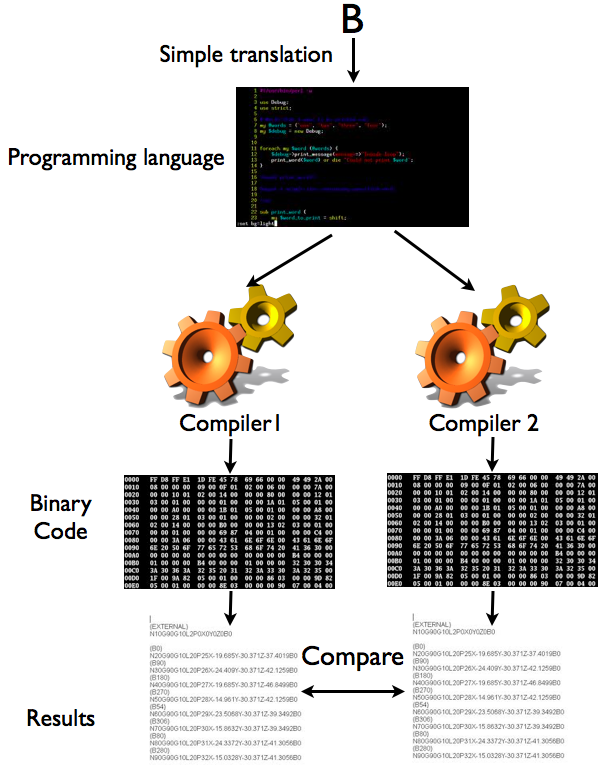
\includegraphics[width=0.70\textheight]{figures/Approach1.png}\\  ~ \\
               %\includegraphics[width=.45\textwidth]{figures/bigStep.jpg}
    \end{center}
    \end{columns}
	
\end{frame}


\begin{frame}
	\frametitle{Goal of this work}
	
	    \begin{columns}[c]
	    \column{.5\textwidth} 
	
		\begin{itemize}
		\item The goal of this work is to connect the B method to the LLVM compilation framework%~\cite{Lattner04LLVM}.
		\note[item]{The goal of this work is provides a safe connection between the B method and the LLVM compilation framework.} 
		\item  LLVM is a free, open-source project which many compiling contemporary technologies.
			\begin{itemize}
			\item Provides an intermediate assembly language (LLVM-IR).
			\item Supports many languages.
			\note[item]{LLVM Languages supported Ruby, Python, Haskell, Java, D, PHP, Pure, Lua}
			\note[item]{LLVM received the prestigious ACM Software Award and it attracted the attention of importants companies.}
			\note[item]{We are working in a subset of LLVM intermediate representation}
			\end{itemize}
		\end{itemize}

    \column{.5\textwidth}
    \begin{center}
               
\includegraphics[width=.5\textwidth]{figures/logoB.png} 
               \\*
               \setlength{\unitlength}{0.3mm}
				\begin{picture}(5,5)
				\put(10,20){\vector(-1,-4){5}}
				\end{picture}
				\\*
               
\includegraphics[width=.5\textwidth]{figures/LLVM-Logo-Derivative-4.png}
    \end{center}
    \end{columns}		
		

\end{frame}


\section{B0 Language}

\begin{frame}[fragile]
\frametitle{Reduced B0 Grammar}

\begin{columns}[t]

\begin{column}[T]{5cm}
	\begin{itemize}
	\item B0 Implementation	
	\end{itemize}	     
     \definecolor{bg}{rgb}{0.87,0.87,0.87}
\footnotesize{
%\begin{minted}[bgcolor=bg]{pascal}
%IMPLEMENTATION
%	counter_i
%	...
%CONCRETE_VARIABLES
%  value, error
%INVARIANT
%  value : INT &
%  error : BOOL 
%INITIALISATION
%  BEGIN
%    value := 0;
%    error := FALSE
%  END
% ...
%\end{minted}
}

  \end{column}

\begin{column}[T]{5cm} 
	\begin{itemize}
	\item Reduced B0 Grammar	
	\end{itemize}	     
%	\includegraphics[scale=0.3]{figures/code/ABS.png}	
\scriptsize{
\begin{sloppypar} 
Clause\_implementation ::=\\
\hspace*{0.20in} $|$ \texttt{Clause\_sees}\\
\hspace*{0.20in} $|$ \texttt{Clause\_imports}\\
\hspace*{0.20in} $|$ \texttt{Clause\_promotes}\\
\hspace*{0.20in} $|$ \texttt{Clause\_extends\_B0} \\
\hspace*{0.20in} $|$ \textcolor{gray}{Clause\_sets}\\
\hspace*{0.20in} $|$ \textbf{Clause\_concrete\_constants}\\
\hspace*{0.20in} $|$ Clause\_properties\\
\hspace*{0.20in} $|$ Clause\_values\\
\hspace*{0.20in} $|$ \textbf{Clause\_concrete\_variables}\\
\hspace*{0.20in} $|$ \textcolor{gray}{Clause\_invariant}\\
\hspace*{0.20in} $|$ \textcolor{gray}{Clause\_assertions}\\
\hspace*{0.20in} $|$ \textbf{Clause\_initialisation\_B0\\
\hspace*{0.20in} $|$ Clause\_operations\_B0}\\
\end{sloppypar}}

\begin{itemize}

%\item B0 is the subset of the B language that is used to describe imperative programs.
\item It is subset of the B language and has only algorithmic constructs.
\end{itemize}



\end{column}


     \end{columns}


%  \caption{Abstract syntax structure of designed B0 implementation. }
  \note[item]{The first common elements are being implemented and should support the modularization.}
  \note[item]{The gray elements are not supported yet.}
  \note[item]{The bold elements are supported in the first prototype B2LLVM.} 
  \note[item]{This work considers currently types INT (integer) and BOOL (Boolean)}	
\end{frame}





 
\frame{
\frametitle{B0 Language} 
\begin{itemize}
%\item B0 is the subset of the B language that is used to describe imperative programs.
%	\item B0 has only algorithmic constructs.
\item An example of syntax tree:
\end{itemize}
	\begin{align*}
&  \underbrace{ \underbrace{BEGIN   \underbrace{\underbrace{\underbrace{value}_\text{\onslide<2->{IDENTIFIER}} :=\underbrace{0}_\text{\onslide<2->{EXPRESSION}} }_\text{\onslide<3->{INSTRUCTION}} ;\underbrace{\underbrace{error}_\text{\onslide<2->{IDENTIFIER}} :=\underbrace{FALSE}_\text{\onslide<2->{EXPRESSION}} }_\text{\onslide<3->{INSTRUCTION}}  }_\text{\onslide<4->{INSTRUCTION}} END}_\text{\onslide<5->{INITIALISATION}}}_\text{\onslide<6->{IMPLEMENTATION}} \\
	\end{align*}

\note[item]{This syntax tree is translated to LLVM-IR} 
}




\section{Target LLVM}

%\begin{frame}
%	\frametitle{Grammar LLVM}
%
%	\begin{figure}[H]
%  		\begin{center}
%		 \includegraphics[scale=0.22]{figures/code/grammar_LLVM.png}	
%		  \caption{Grammar target LLVM. }
%		      \note[item]{This is the LLVM grammar subset.}
% 	    \label{fig:grammarLLVM}
%        \end{center}
%     \end{figure}
%\end{frame}


%\begin{frame} \frametitle{Simplified Translation}
%
%	\begin{figure}[H] \begin{center}
%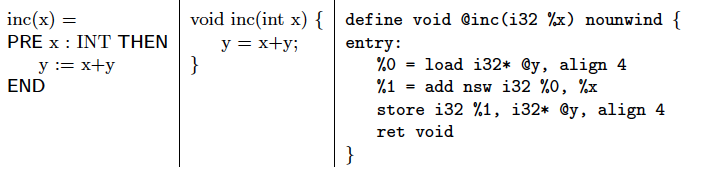
\includegraphics[scale=0.4]{figures/code/B_C_LLVM.png}	\caption{A simplified
%example of translation \textbf{B0}, \textbf{C} and \textbf{LLVM}. }
%\note[item]{This example just illustrate the similarity of code and the
%strategy of translation.} \label{tab:grammarLLVM} \end{center} \end{figure}
%
%	   \begin{block}{Attention} This example is minimal and very
%simplified, the real translation has many translation rules from B to LLVM.
%\end{block} \note[item]{ The B language has defined a subset of implementable
%algorithms constructs, called B0} 
%	\note[item]{The body of code use static single assignment form that is a property of an intermediate representation (IR), which says that each variable is assigned exactly once}   		 
%\end{frame}


\begin{frame} \frametitle{LLVM-IR}

	\begin{itemize}
	\item The LLVM has an assembly language that provides intermediate representation (IR)
		\begin{itemize}
			\item uses static single assignment 
			\item is strongly typed 
		\note[item]{Every value has a type (getType()) 
	and a value must be explicitly cast to a new type}
		\end{itemize}
	\note[item]{which says that each variable is assigned exactly once.}
%	\item Suppose infinity variables memory 

	\item Groups of translation rules from B0 to LLVM were developed based on B0 Grammar.
	\end{itemize}
	
\end{frame}




\section{Translation}



\begin{frame}
	\frametitle{Rule Groups of Translation}

\begin{itemize}
\item The translation of the different elements of a B
implementation is divided into:
	\begin{itemize}
	\item \textbf{Modularity} constructs to combine B components (SEES, INCLUDES, IMPORTS).
	\item \textbf{Data} translation, including the encoding of B data types.
	\note[item]{Let`s see an example of data translation.}
	\item \textbf{Expressions} and \textbf{conditions} are codified as LLVM instruction block.
	\item \textbf{Control flow} are translated to LLVM control flow statements.
	\note[item]{ The control flow instructions are translated to LLVM control flow statements, which also supports the encoding of B operations and initialisation}
	\end{itemize}
\end{itemize}

\end{frame}




\begin{frame}[fragile]
\frametitle{Initialisation B0 and LLVM-IR }
\definecolor{bg}{rgb}{0.87,0.87,0.87}

\begin{itemize} \item B0
\end{itemize}
\scriptsize{
%\begin{minted}[bgcolor=bg]{pascal}
%
%BEGIN 
%    value := 0;
%    error := FALSE
%END
%\end{minted}
}

\begin{itemize} \item LLVM-IR
\end{itemize}

\scriptsize{
%\begin{minted}[bgcolor=bg,mathescape]{nasm}
%
%%counter_i$\char36$state$\char36$ = type {i32, i1}
%define void @counter_i$init$(%counter_i$state$* %self$) {
%entry:
%  %0 = getelementptr %counter_i$state$* %self$, i32 0, i32 0
%  store i32 0, i32* %0
%  %1 = getelementptr %counter_i$state$* %self$, i32 0, i32 1
%  store i1 0, i1* %1
%  br label %exit
%exit:
%  ret void
%
%\end{minted}
}

\end{frame}







%
%\begin{frame}[fragile]
%\frametitle{B Code - Initialisation}
%
%\definecolor{bg}{rgb}{1,1,1}
%\footnotesize{
%\begin{minted}[bgcolor=bg]{pascal}
%IMPLEMENTATION
%	counter_i
%	...
%CONCRETE_VARIABLES
%  value, error
%INVARIANT
%  value : INT & error : BOOL 
%INITIALISATION
%  BEGIN
%    value := 0;
%    error := FALSE
%  END
% ...
%\end{minted}
%}
%\end{frame}

%\begin{frame}[fragile]
%\frametitle{Implemention  Rule }
%
%\definecolor{bg}{rgb}{1,1,1}
%\scriptsize{
%\begin{minted}[bgcolor=bg]{python}
%def translate_implementation(i):
%    '''
%    - Input:
%      i: a node representing a B implementation
%    - Output:
%      The text of the LLVM encoding for i.
%    '''
%    check_kind(i, {"Impl"})
%    result = ""
%    result += translate_type_def_import_list(i)
%    result += translate_op_decl_import_list(i)
%    result += translate_constants(i)
%    result += translate_state(i)
%->  result += translate_init(i)
%    for op in i["operations"]:
%        result += translate_operation(op)
%    return result
%\end{minted}
%}
%
%\end{frame}



\begin{frame}[fragile]
\frametitle{Current State of B2LLVM}
	\begin{figure}[H]
               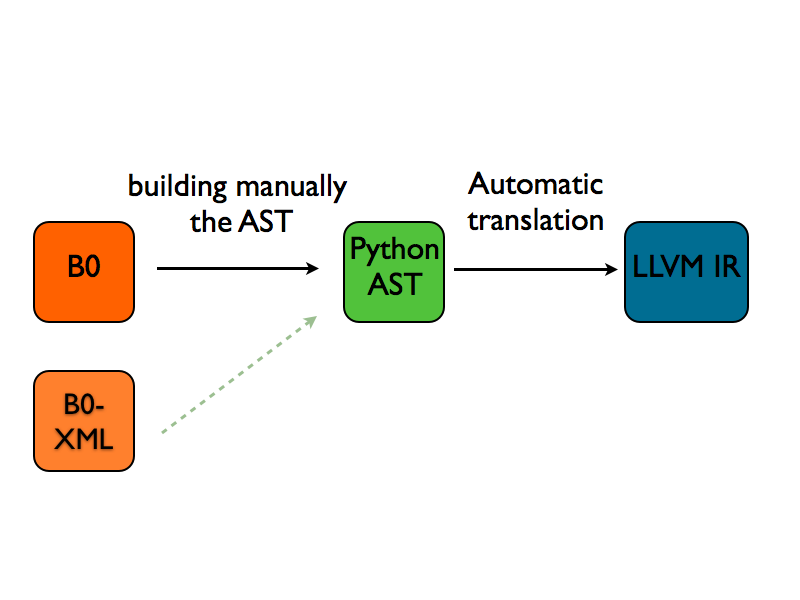
\includegraphics[width=.777\textwidth]{figures/CurrentState.png} 
	\end{figure}
\end{frame}

%\begin{frame}[fragile]
%\frametitle{Rule Python}
%
%\definecolor{bg}{rgb}{1,1,1}
%\scriptsize{
%\begin{minted}[bgcolor=bg]{python}
%
%def translate_init(i):
%    '''
%    Input:
%      - i: root node of a B implementation AST
%    Output:
%    LLVM implementation of the initialisation clause of i (a LLVM function).
%    '''
%    global tb, nl, sp
%    check_kind(i, {"Impl"})
%    reset_llvm_names()
%    result = "define void" + sp + init_name(i) 
%    result += "("+state_t_name(i)+"* %self$) {" + nl
%    result += "entry:" + nl
%    result += translate_alloc_inst_list(i["initialisation"])
%    result += translate_import_init_list(i)
%    result += translate_inst_list_label(i["initialisation"], "exit")
%    result += "exit:" + nl
%    result += tb + "ret void" + nl
%    result += "}" + nl
%    return result; 
%
%\end{minted}
%}
%\end{frame}







%\begin{frame}
%	\frametitle{Translation rules (high level)}
%
%	\begin{figure}[H]
%  		\begin{center}
%		 \includegraphics[scale=0.3]{figures/code/imp.png}	\\
%		 \includegraphics[scale=0.27]{figures/code/oper.png}\\
% 		 %\includegraphics[scale=0.25]{figures/code/inst.png}	
%		  \caption{Implementation and operation rules}
%		  % \note[item]{.}
%        \end{center}
%     \end{figure}
%
%\end{frame}
%
%\begin{frame}
%	\frametitle{Translation rules (low level)}
%
%	\begin{figure}[H]
%  		\begin{center}
%		 \includegraphics[scale=0.25]{figures/code/inst.png}	
%		 %TODO complement the rules to understand better
%		  \caption{Instructions.}
%		  % \note[item]{.}
%		\note[item]{These rules are the most important, there are several other, but the presentation time is short}
%        \end{center}
%     \end{figure}
%\end{frame}
%

\section{Conclusion}



\begin{frame}
	\frametitle{Conclusion and Future Work}
	\begin{itemize}
	\item This paper presents the specification of a \textbf{translation} from a large subset of the B implementation language to LLVM
 \note[item]{a modern compiler internal language.}
 	
\item  Even though this is still a\textbf{ work in progress}, the definition has a \textbf{large enough scope} to be applied to B implementations where the data belongs to basic types. %This specification is a blueprint for a code synthesis tool for B that is currently being implemented. 
	\item This tool will be distributed under an \textbf{open-source license}.
	\note[item]{This tool will be compatible with the next version of AtelierB.} 
	\end{itemize}
\end{frame}

\begin{frame} \frametitle{Conclusion and Future Work}
	 \begin{itemize}
	 \item Verify the translation
	\begin{itemize} 
	\item Define the semantics of LLVM and B in a unified framework. 
	 \item Possibles approaches:
	\begin{itemize} 
	\item Take advantage of Vellvm, a framework to reason about
correctness of LLVM. 
	 \item Translate verification conditions from B development artifacts as assertions in LLVM code.
	\item Use an automatic test generator and apply to generated code.
	\end{itemize}
	\end{itemize} 
	\end{itemize} 
\end{frame}


\begin{frame}

\frametitle{Acknowledgments}
\center{Thank you for your attention!} \\ ~ \\

\includegraphics[width=.2\textwidth]{figures/cnpq.jpg}\ \ \ \ \ \ \ \ 

\includegraphics[width=.25\textwidth]{figures/ines.png} \\ ~ \\

\includegraphics[width=.2\textwidth]{figures/ifrn.jpeg}\ \ \ \ \ \ \ \

\includegraphics[width=.2\textwidth]{figures/ufrn.jpeg}

\end{frame}


\begin{frame}
  \frametitle{References}

  \begin{thebibliography}{10}

  \beamertemplatearticlebibitems

  \bibitem{Abrial}
    J.-R. Abrial. 
   \newblock {The B-book: assigning programs to meanings. Cambridge University Press, 1996.}

  \bibitem{B method}
    B Method
    \newblock {\tt http://www.atelierb.eu/en/}

  \bibitem{LLVM}
    The LLVM Compiler Infrastructure
    \newblock {\tt http://llvm.org/}

  \bibitem{Vellvm}
    Jianzhou Zhao, Santosh Nagarakatte, Milo M. K. Martin, and Steve Zdancewic.
   Formalizing the LLVM intermediate representation for verified program transformations. In POPL, pages 427–440, 2012.
    \newblock {\tt http://www.cis.upenn.edu/\~\ stevez/vellvm/}

  \end{thebibliography}
\end{frame}









\end{document}
